\documentclass[11pt, a4paper]{article}
\usepackage[utf8]{inputenc}
\usepackage[english]{babel}
\usepackage{amsmath}
\usepackage{amsthm}
\usepackage{amsfonts}
\usepackage{amssymb}
\usepackage{graphicx}
\usepackage{tikz}
\usepackage{listings}
\usepackage[justification=centering]{caption}
\usetikzlibrary{arrows, automata, graphs, shapes, petri, decorations.pathmorphing}

% define environments
\theoremstyle{definition}
\newtheorem{definition}{Definition}

\theoremstyle{plain}
\newtheorem{theorem}[definition]{Theorem}
\newtheorem{lemma}[definition]{Lemma}

\renewcommand{\labelenumi}{(\roman{enumi})}

\author{Niklas Rieken}
\title{Von Pushdown-Automaten\\zu kontextfreien Grammatiken}


\begin{document}
\maketitle
Die Definition 7.24 aus der Vorlesung (s. Abbildung~\ref{fig:pda2cfg}) beschreibt, wie sich aus einem Pushdown-Automaten, der mit leerem Stack akzeptiert eine kontextfreie Grammatik konstruieren lässt, die die selbe Sprache erzeugt. Das Verfahren ist eigentlich sehr einfach, allerdings ist die Funktionsweise nicht sehr intuitiv, da sich die Produktionsregeln der erzeugten Grammatik nicht so leicht interpretieren lassen (oder: sie lassen sich nicht so einfach von links nach rechts lesen).\par
\begin{figure}
	\centering
	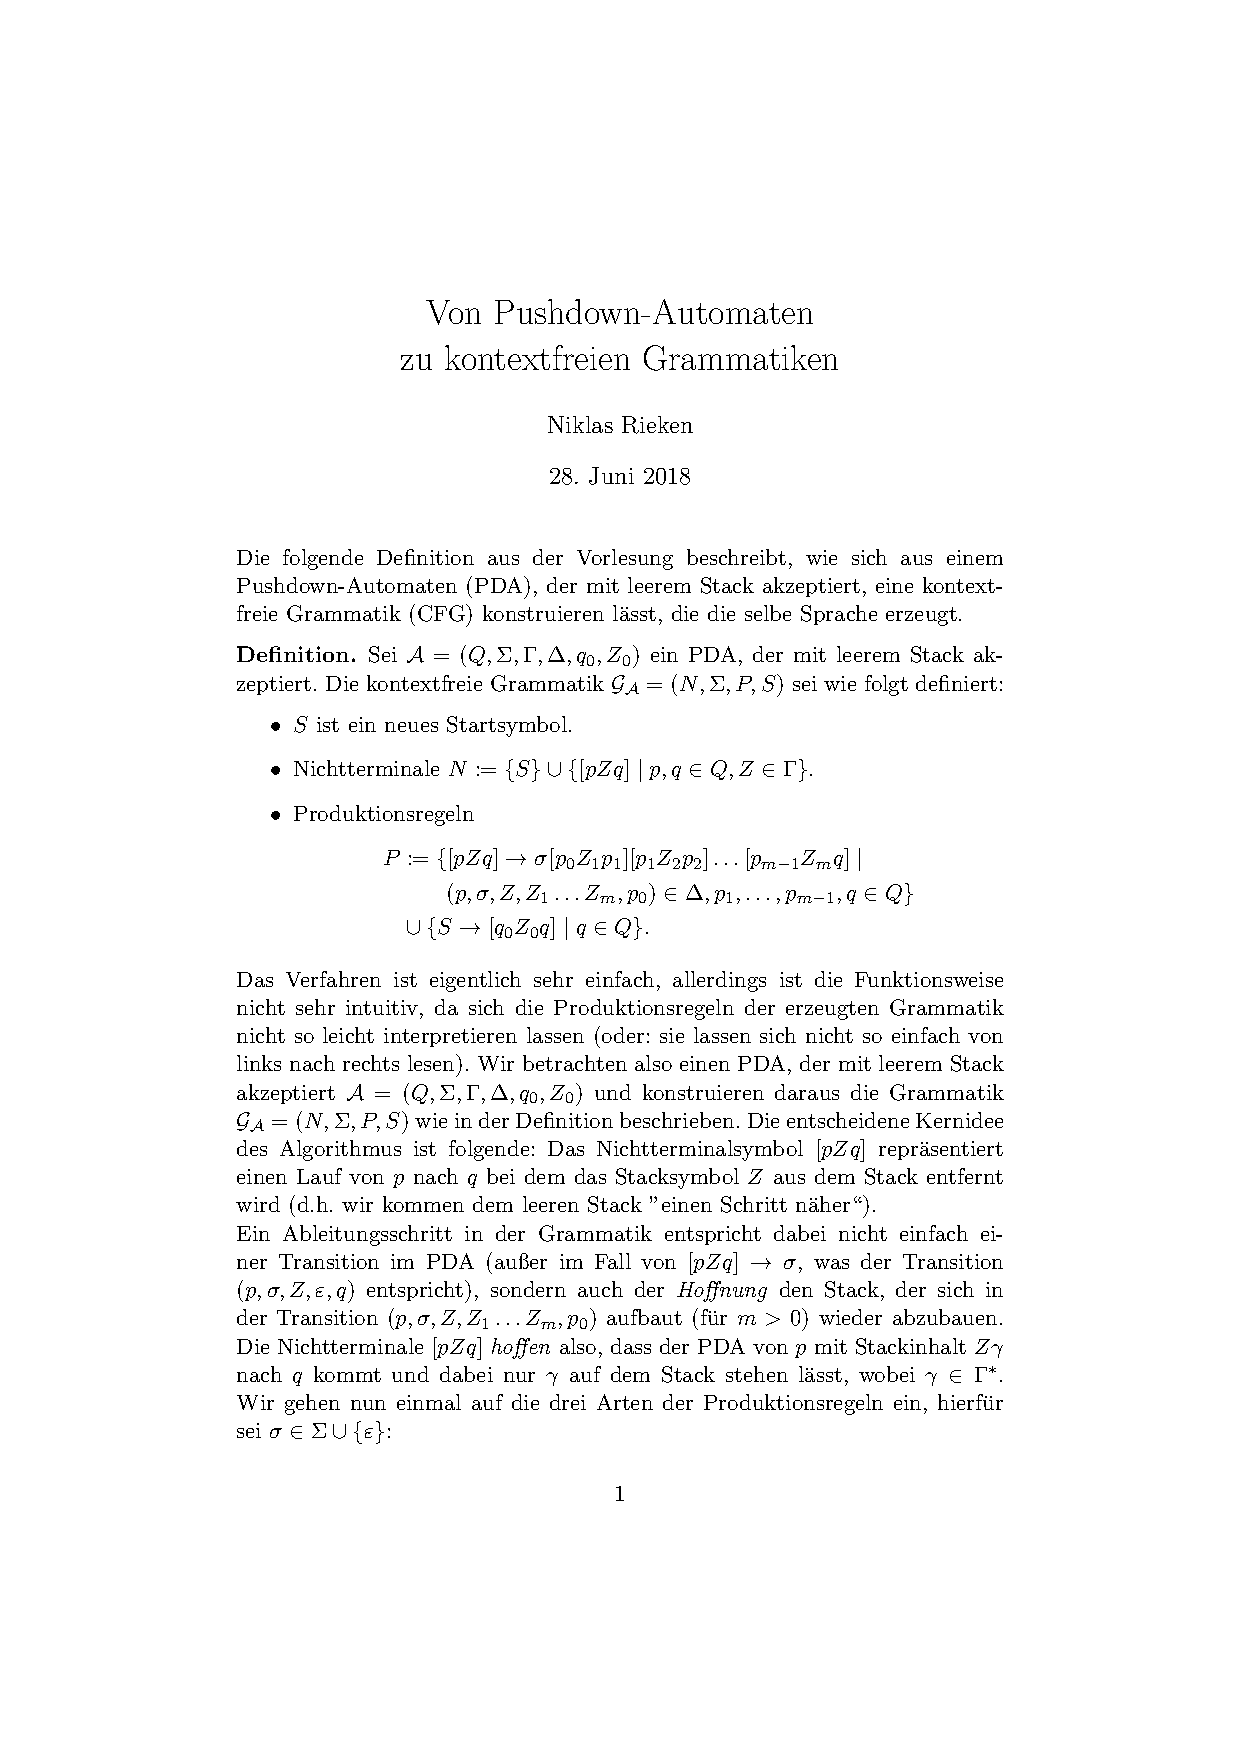
\includegraphics[scale=.3]{pda2cfg.png}
	\caption{Definition 7.24 aus der Vorlesung.}
	\label{fig:pda2cfg}
\end{figure}
Wir betrachten also einen PDA, der mit leerem Stack akzeptiert \( \mathcal{A} = (Q, \Sigma, \Gamma, \Delta, q_0, Z_0) \) und konstruieren daraus die Grammatik \( \mathcal{G_A} = (N, \Sigma, P, S) \) wie in Abbildung~\ref{fig:pda2cfg} beschrieben. Die entscheidene Kernidee des Algorithmus ist folgende: Das Nichtterminalsymbol \( [pZq] \) repräsentiert einen Lauf von \( p \) nach \( q \) bei dem das Stacksymbol \( Z \) aus dem Stack entfernt wird (d.h. wir kommen dem leeren Stack ''einen Schritt näher``).\\
Ein Ableitungsschritt in der Grammatik entspricht dabei nicht einfach einer Transition im PDA (außer im Fall von \( [pZq] \to \sigma \), was der Transition \( (p, \sigma, Z, \varepsilon, q) \) entspricht), sondern auch der \textit{Hoffnung} den Stack, der sich in der Transition \( (p, \sigma, Z, Z_1 \ldots Z_k, p_0) \) aufbaut (für \( k > 0 \)) in einer der Zukunft wieder abzubauen. Die Nichtterminale \( [pZq] \) \textit{hoffen} also, dass der PDA von \( p \) mit Stackinhalt \( Z\gamma \) nach \( q \) kommt und dabei nur \( \gamma \) auf dem Stack stehen lässt, wobei \( \gamma \in \Gamma^\ast \). Wir gehen nun einmal auf die drei Arten der Produktionsregeln ein, hierfür sei \( \sigma \in \Sigma \cup \{ \varepsilon \} \):
\begin{itemize}
	\item Mit dem Startsymbol \( S \) haben wir folgende Produktionsregeln: \( S \to [q_0 Z_0 q] \) \textbf{für alle} \( q \in Q \).\\
	Die Akzeptanzbedingung des Automatenmodells ist allein vom Stack abhängig, in welchem Zustand ein Lauf terminiert ist also egal, deswegen bilden wir diese Regel für jedes \( q \). Hier rufen wir uns nochmal die Intuition der Nichtterminale (außer \( S \)) in Erinnerung: Gesucht wird also ein Lauf auf \( \mathcal{A} \) vom Startzustand \( q_0 \) zu einem beliebigen \( q \), sodass das Bottom-of-Stack-Symbol \( Z_0 \) weggenommen wird (d.h. nur noch \( \varepsilon \) auf dem Stack steht). Diese Regeln sind drücken also genau unseren gewünschten Lauf aus: Von der Startkonfiguration \( (q_0, Z_0) \) zu einer Konfiguration \( (q, \varepsilon) \).
	\item Für die Transitionen der Form \( (p, \sigma, Z, \varepsilon, q) \) erhalten wir die Produktionsregel \( [pZq] \to \sigma \). Dies sind die Regeln in denen der Stack tatsächlich abgebaut wird ohne ihn vorher zu erweitern (s. nächster Punkt).
	\item Regeln der Form \( [pZp_m] \to \sigma [p_0 Z_1 p_1][p1 Z_2 p_2] \ldots [p_{m-1} Z_m p_m] \) für eine Transition \( (p, \sigma, Z, Z_1 \ldots Z_m, p_0) \in \Delta \) und \textbf{alle möglichen(!)} Zustände \( p_1, \ldots, p_m \in Q \):\\
	Dies ist die schwerste Art der konstruierten Produktionsregeln. Wir versuchen dies trotzdem einmal in einem Satz von links nach rechts zu beschreiben, auch wenn das etwas konstruiert wirkt:
	Wir befinden uns in Zustand \( p \) mit \( Z \) oben auf dem Stack, welches wir entfernen wollen, und dabei den Zustand \( p_m \) erreichen mit einer Transition über \( \sigma \), wo wir den Stack mit \( Z_1, \ldots, Z_m \) auffüllen, welche wir dann in der Zukunft, d.h. in einem Lauf über \( p_0 \) bis \( p_m \), abbauen müssen über weitere Regeln dieser Form und -- schlussendlich -- über Regeln der Art aus dem vorigen Punkt.\\
	Eine Ableitung eines Wortes repräsentiert also genau einen akzeptierenden (d.h. mit \( \varepsilon \) auf dem Stack am Ende) Lauf auf dem PDA.
\end{itemize}
Um die Philosophie der Konstruktion einmal zusammenzufassen: Wenn in einem akzeptierenden Lauf der aktuelle Stackinhalt zu einem Zeitpunkt \( Z\gamma \) ist, dann wird zu einem späteren Punkt des Laufes der Stackinhalt einmal nur noch \( \gamma \) sein.\\
Wir betrachten als Beispiel den PDA, der mit leerem Stack akzeptiert in Abbildung~\ref{fig:pda}. Sei dafür 
\[
	\mathcal{A} = (\{ p, q \}, \{ a, b \}, \{ Z \}, \{(p, a, Z, ZZ, p), (p, a, Z, Z, q), (q, b, Z, \varepsilon, q) \}, p, Z). 
\]
\begin{figure}
	\centering
	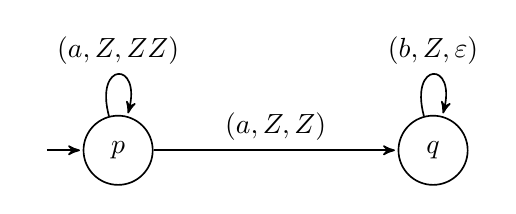
\begin{tikzpicture}[->, >=stealth', shorten >=1pt, auto, semithick]
		\node[initial, state, initial text=] (p) at (0, 0) {$p$};
		\node[state] (q) at (4, 0) {$q$};
		
		\path (p) edge node {$(a, Z, Z)$} (q)
			(p) edge[loop above] node {$(a, Z, ZZ)$} (p)
			(q) edge[loop above] node {$(b, Z, \varepsilon)$} (q);		
	\end{tikzpicture}
	\caption{PDA, der mit leerem Stack akzeptiert für die Sprache \( L = \{ a^n b^n : n \in \mathbb{N}_+ \} \).}
	\label{fig:pda}
\end{figure}
Wir erhalten zunächst für die Grammatik \( \mathcal{G_A} = (N, \{ a, b \}, P, S) \) mit \( N = \{ S, [pZp], [pZq], [qZp], [qZq] \} \). Die Produktionsregeln \( P \) konstruieren wir nacheinander:
\begin{itemize}
	\item Zunächst ist es uns egal in welchem Zustand wir terminieren (auch wenn ein akzeptierender Lauf offensichtlich nur in \( q \) enden kann), die einzige Bedingung, die wir an den Lauf stellen ist, dass er im Startzustand \( p \) beginnt mit dem Bottom-of-Stack-Symbol \( Z \) oben auf dem Stack. Insgesamt erhalten wir also die Regeln
	\[
		S \to [pZp] \,\vert\, [pZq] \in P.
	\]
	\item Nun betrachten wir die Transitionen, die den Stack abbauen. Davon gibt es nur eine im Loop über \( q \), d.h. \( (q, b, Z, \varepsilon, q) \). Wir erhalten also:
	\[
		[qZq] \to b \in P.
	\]
	\item Zuletzt noch die Transitionen, die den Stack vorübergehend aufbauen. Für die Transition \( (p, a, Z, ZZ, p) \) erhalten wir die Regeln
	\begin{align*}
		[pZp] &\to a[pZp][pZp] \,\vert\, a[pZq][qZp],\\
		[pZq] &\to a[pZp][pZq] \,\vert\, a[pZq][qZq] \in P
	\end{align*}
	und für die Transition \( (p, a, Z, Z, q) \) nur die Regel
	\[
		[pZq] \to a[qZq] \in P.
	\]
	\item Wir stellen fest, nachdem wir alle Regeln aus den Transitionen gebaut haben, dass die Regel  \( [pZp] \to a[pZq][qZp] \) weggelassen werden kann, da wir keine Regel mit \( [qZp] \) als linker Seite haben. Ein Anwenden dieser Regel könnte also nicht terminieren. Dies ist auch intuitiv klar, da ein Lauf von \( q \) nach \( p \) -- unabhängig vom Stackinhalt -- nicht möglich ist.
\end{itemize}
\end{document}
